\documentclass[../main]{subfiles}
\graphicspath{{\string~/AQUOS/Default_Folder/TIU/lectures/05_R/tex/fig/}}
\begin{document}

\tcbstartrecording\relax

\section{描画用データ作成}

\Definition{手順}
{
  描画用データとして,平均,標準偏差が異なる3種類の正規乱数(N=100)を作成する.\\
  また,表示用の色をそれぞれ作成する.
}

\lstinputlisting[firstline=1,lastline=21]{\DirCourse/05_R/tex/fig/graph.r}

\begin{exercise}
  上記のソースコードを「graph.r」として保存してください.\\
  色彩名表示\cs{colors()}でどのような色があるか確認してください.
  %「R」,「色見本」,「colors」などのキーワードで,
  %インターネットでどのような色見本があるか検索してください.

 色彩名 -> RGB変換: \cs{col2rgb('色彩名')}\\
 色彩名関数: \cs{rainbow(n)}, \cs{heat.colors(n)}, \cs{grey(1:11/12)},\\\hfill
  \cs{terrain.colors(n)}, \cs{topo.colors(n)}, \cs{cm.colors(n)}\\
 cf. \href{https://oku.edu.mie-u.ac.jp/~okumura/stat/colors.html}{奥村研究室,「統計グラフの色」}
  \tcblower
\end{exercise}

\section{散布図}

\lstinputlisting[firstline=3,lastline=21]{\DirCourse/05_R/tex/fig/050-scatter.r}

\begin{exercise}
  グラフィックオプションは次のようなものがあります.\\
  値を変更してグラフを変化させてみてください.\\ \relax
  \cs{type}=\{p, l, b, o, s, h, n\},
  \cs{pch}=0--25, 
  \cs{lty}=0--6
\tcblower
\end{exercise}

\begin{figure}[H]
  \centering
  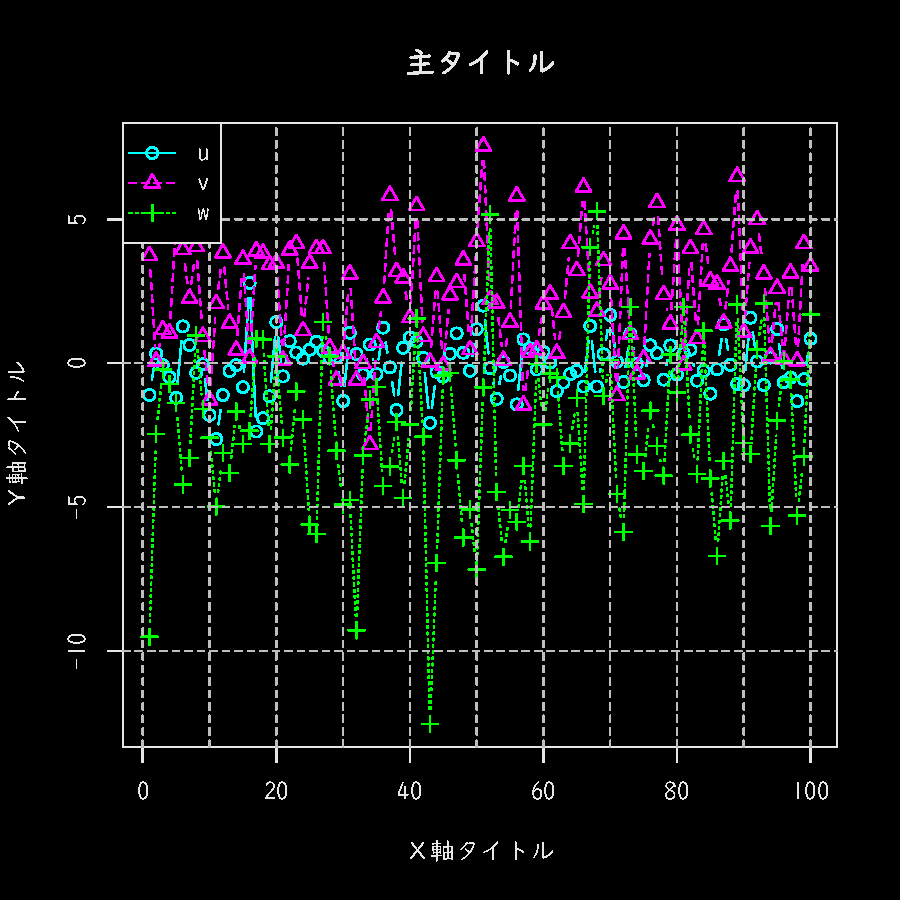
\includegraphics[height=0.9\textheight]{scatter}
  \caption{散布図描画例}
  \label{fig:scatter}
\end{figure}

\ctable[pos=H,caption=\cs{plot}オプション一覧]{ll}{}
{
  \FL
  オプション名& 内容\ML
  \cs{type}   & plot \textbf{type}\NN
  \cs{col}    & plot \textbf{col}or\NN
  \cs{bg}     & \textbf{b}ack\textbf{g}round color\NN
  \cs{pch}    & \textbf{p}oint \textbf{ch}aracter\NN
  \cs{lty}    & \textbf{l}ine \textbf{ty}pe\NN
  \cs{lwd}    & \textbf{l}ine \textbf{w}i\textbf{d}th\NN
  \cs{h}      & \textbf{h}orizontal line\NN
  \cs{v}      & \textbf{v}ertical line\LL
}

\section{ヒストグラム}

\begin{ConsoleR}
cairo_pdf('fig/hist.pdf', width = 6, height = 6, family = "UDDigiKyokashoN-R")

# データ
source('graph.r')
# dark.theme()

# ヒストグラムのビン
b <- seq(-20, 20, 1)

# 枠
hist(d@\$@u, breaks=b, col=0, border=0, main='主タイトル', xlab='軸タイトル', ylab='度数')

(次へ続く)
\end{ConsoleR}

\begin{ConsoleR}
(前からの続き)

# 罫線
abline(h=seq(0,50,10),col=8,lty=2)

# プロット
hist(d@\$@u, breaks=b, col=RGBS[1], add=T)
hist(d@\$@v, breaks=b, col=RGBS[2], add=T)
hist(d@\$@w, breaks=b, col=RGBS[3], add=T)

# 凡例
legend('topleft', legend=c('u','v','w'), fill=RGBS)

dev.off()
\end{ConsoleR}

\begin{figure}[H]
  \centering
  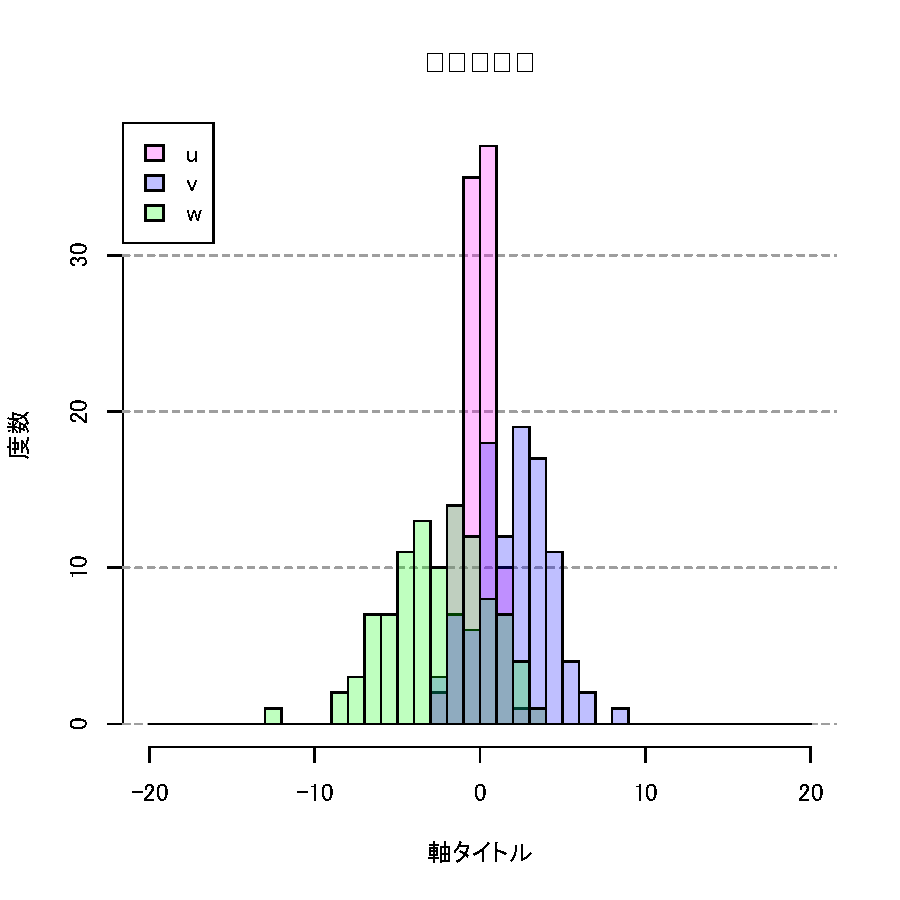
\includegraphics[height=0.9\textheight]{hist}
  \caption{ヒストグラム描画例}
  \label{fig:hist}
\end{figure}

\cs{add = T} オプションで重ね書きができる\\
\cs{rgb(red = 0, blue = 1, green = 0, alpha = .5)}\\
      \hfill でRGB値を出力できる(alpha: 透明度)

\section{回帰モデルグラフ}

\begin{ConsoleR}
cairo_pdf('fig/lm.pdf', width = 6, height = 6, family = "UDDigiKyokashoN-R")

# 枠設定
matplot (x.all, y.fit, type='n', xaxt='n', yaxt='n', main='主タイトル', xlab='X軸タイトル', ylab='Y軸タイトル')
# プロット
matpoints(x.obs, y.obs, col=2, pch=1) # 観測値
matlines (x.all, y.true,col=2, lty=1) # 真値
matlines (x.all, y.fit, col=4, lty=1) # 予測値
matlines (x.all, y.upr, col=4, lty=2) # 上限値
matlines (x.all, y.lwr, col=4, lty=2) # 下限値
abline(v=n.obs, col='gray', lty=2)
(次へ続く)
\end{ConsoleR}

\begin{ConsoleR}
(前からの続き)
# 軸設定
axis(1, at    = seq(0, n.all, 2), # X軸配置
        label = seq(0, n.all, 2)) # ラベル
axis(2, at    = seq(0, 900, 100), # Y軸配置
        label = seq(0, 900, 100)) # ラベル 
# 凡例設定
legend('topleft', # 表示位置
  legend = c('観測値', '真値',
             '予測値', '95%予測区間'),
  col    = c( 2,  2,  4,  4), # 色
  pch    = c( 1, NA, NA, NA), # 点種
  lty    = c(NA,  1,  1,  2)) # 線種

dev.off()
\end{ConsoleR}

\begin{figure}[H]
  \centering
  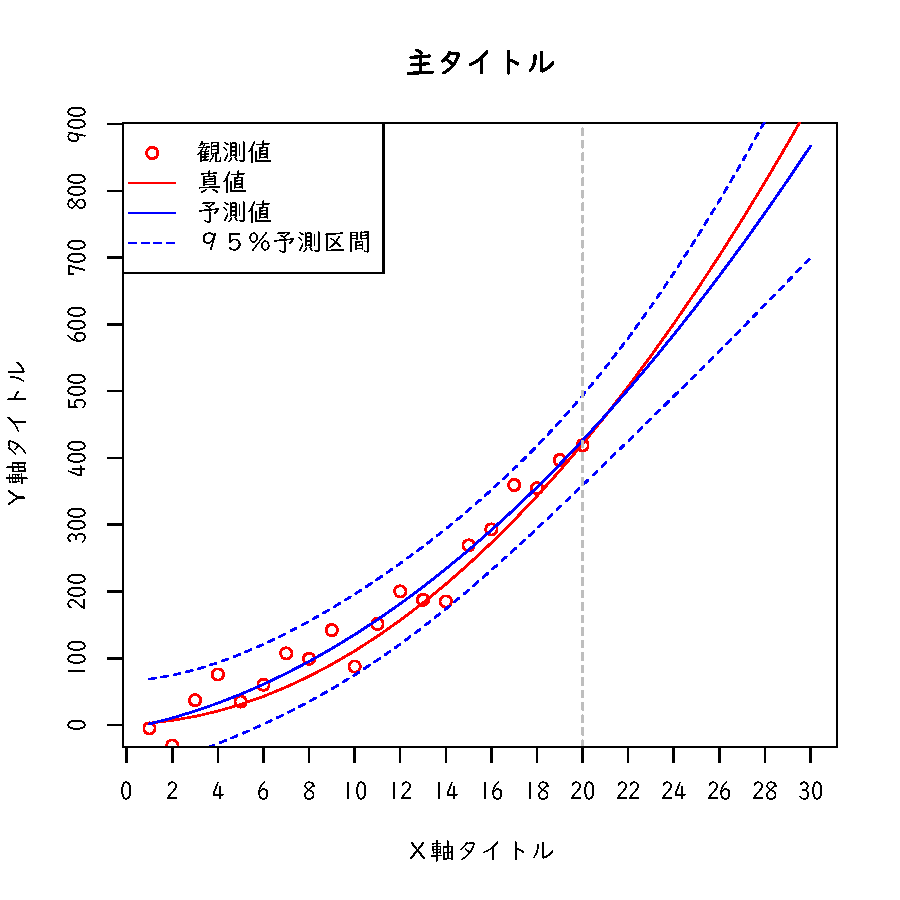
\includegraphics[height=0.9\textheight]{lm}
  \caption{回帰モデルグラフ描画例}
  \label{fig:lm}
\end{figure}
\vspace{-13mm}
描画関数\cs{matpoints}: 点,\cs{matlines}: 線,\cs{abline}: 縦横線,
\cs{axis}: 軸,\cs{legend}: 凡例
描画オプション\cs{col}: 色,\cs{pch}: 点種,\cs{lty}: 線種,
\cs{v}:縦線,\cs{h}:横線

\subsection{テキストデータの出力}

\Definition{手順}
{
  write.csv関数を使用して,オブジェクトデータを
  ファイルにCSVファイル形式*で書き込む.
  * CSV:カンマ区切
} 

\begin{ConsoleR}
d0 <- data.frame(name = c('panda', 'lion'),
                  age = c(5, 7))
write.csv(d0, file = 'd0.csv')
\end{ConsoleR}

\cs{quote = F}オプションをつけると文字列引用符「"」を削除できる.
\cs{write.csv(d0, file = 'd0.csv', quote = F)}

\begin{exercise}
  データフレームを作成し,ファイルに出力してください.
\tcblower
\end{exercise}

\subsection{テキストデータの入力}

\Definition{手順}
{
  read.csv関数を使用して,CSVファイルを読み込み
  オブジェクトに格納する.
}

\begin{ConsoleR}
  d1 <- read.csv(file = 'd0.csv')
  str(d1)
\end{ConsoleR}

\cs{stringsAsFactors} = Fオプションをつけると文字列の自動因子化を抑制します.
\cs{read.csv(file = 'd0.csv', stringsAsFactors = F)}

\begin{exercise}
  CSVファイルを読み込み,オブジェクトに格納してください.
\tcblower
\end{exercise}

\subsection{\Excel データの入力}

\Definition{手順}
{
  excel.linkパッケージを利用し,\R とリンクさせる.\\
  パッケージの利用コマンド: library(excel.link)
}

\begin{exercise}
  \begin{ConsoleR}
  library(excel.link)

  xl.workbook.open('test.xlsx') # Excelを開く
  d <- data.frame(x=3:1, y=-1:1)

  # Sheet1のA1を起点としてデータを書き込み
  xl['Sheet1!A1'] <- d

  # Sheet1のB2からデータを読み込み
  xl['Sheet1!B2'] -> x

  xl.workbook.save('test.xlsx') # Excelを保存
  \end{ConsoleR}
\tcblower
\end{exercise}

xlr: 行名付き,xlc:列名付き, xlrc:行列名付き入出力

\begin{exercise}
  パッケージのヘルプにあるサンプルコードを用いてExcelを操作してください.
\tcblower
\end{exercise}

%=================================================================
\tcbstoprecording
\section{解答}
\tcbinputrecords

\end{document}
